\begin{homeworkProblem}
    \textit{Complex eigenvalues}. Solve and graph the  solutions to the following
    difference equations.
    \begin{enumerate}
        \item $x_{n+2} + x_n = 0$,
        \item $x_{n+2} - x_{n+1} + x_n = 0$,
    \end{enumerate}

    \segline

    \solution

    \begin{enumerate}
        % Solution 9(a)
        \item The characterictic equation is \[
            \lambda^2 + \lambda = 0,
        \]
        with the complex conjugate roots $\lambda = 0 \pm i$. Thus $a=0$ and $b=1$,
        so that \[
            \begin{aligned}
                r = \sqrt{a^2 + b^2} = 1,\\
                \theta = \tan^{-1}(1/0) = \pi/2.
            \end{aligned}
        \]
        Thus the real-valued solution is \[
            x_n = C_1 \cos (n\pi/2) + C_2 \sin (n\pi/2)
        \]
        \begin{figure}[H]
            \centering
            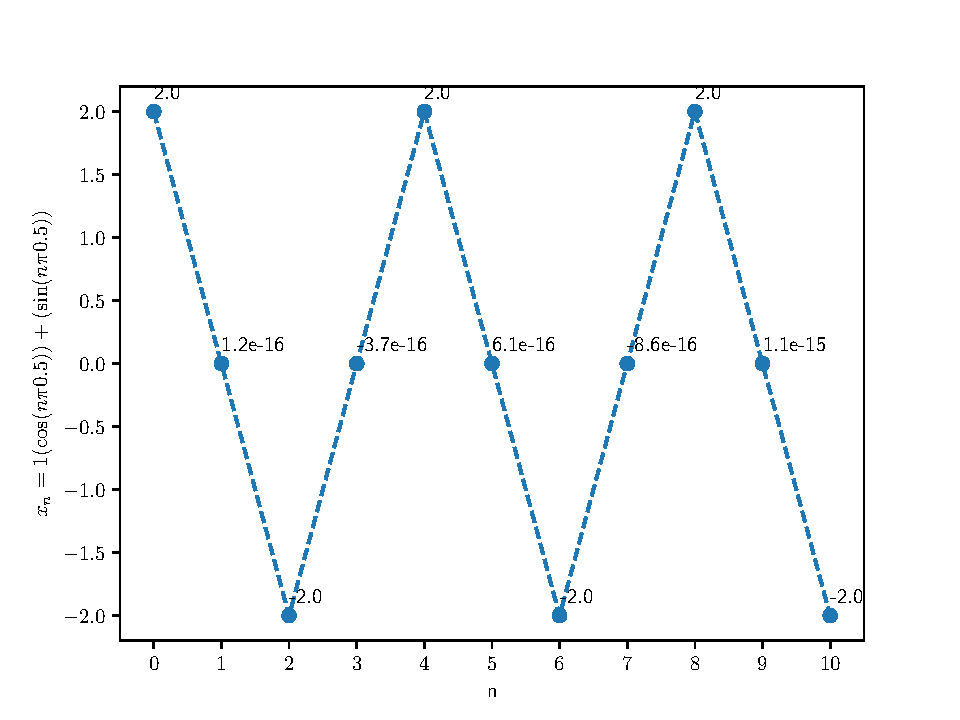
\includegraphics[scale=0.5]{fig/fig9(a).pdf}
        \end{figure}

        % Solution 9(b)
        \item The characterictic equation is \[
            \lambda^2 - \lambda + 1 = 0,
        \]
        with the complex conjugate roots
        $\lambda = \frac{1}{2} \pm \frac{\sqrt{3}}{2}i$.
        Thus $a = \frac{1}{2}$ and $b = \frac{\sqrt{3}}{2}$,
        so that \[
            \begin{aligned}
                r = \sqrt{a^2 + b^2} = 1,\\
                \theta = \tan^{-1}(b/a) = \pi/3.
            \end{aligned}
        \]
        Thus the real-valued solution is \[
            x_n = C_1 \cos (n\pi/3) + C_2 \sin (n\pi/3)
        \]
        \begin{figure}[H]
            \centering
            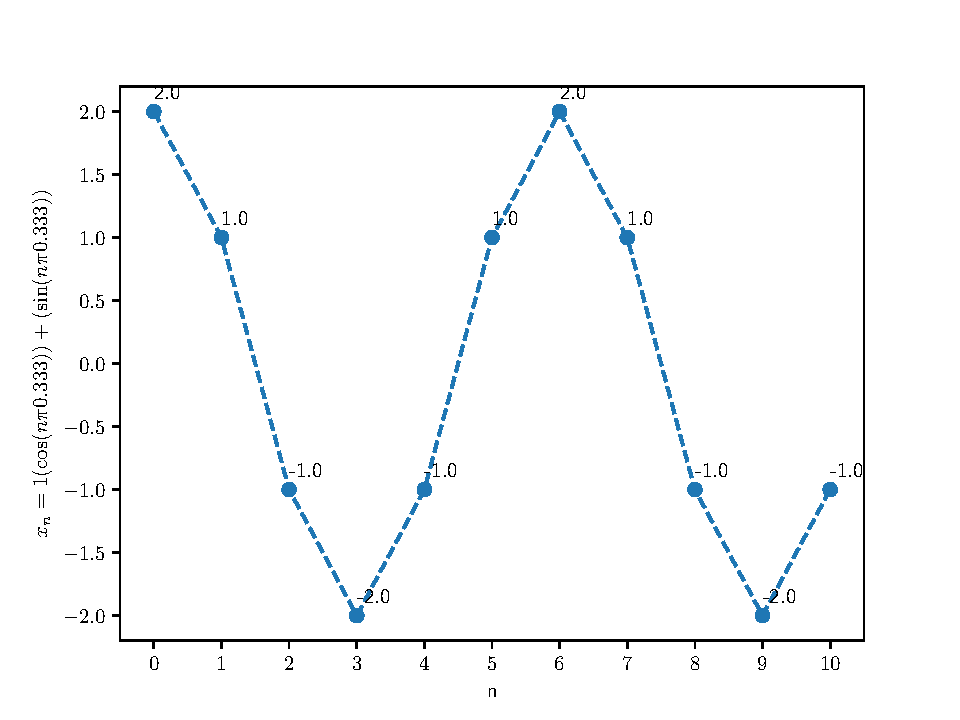
\includegraphics[scale=0.5]{fig/fig9(b).pdf}
        \end{figure}

    \end{enumerate}
    \end{homeworkProblem}